\documentclass[11pt]{article}

\usepackage[margin=1in]{geometry}
\usepackage{amsmath,amssymb}
\usepackage{booktabs}
\usepackage{multirow}
\usepackage{graphicx}
\usepackage{float}
\usepackage{xcolor}
\usepackage{microtype}
\usepackage[numbers,sort&compress]{natbib}
\usepackage[font=small,labelfont=bf]{caption}
\PassOptionsToPackage{hyphens}{url}
\usepackage[colorlinks=true,linkcolor=blue!50!black,citecolor=blue!50!black,urlcolor=blue!50!black]{hyperref}
\Urlmuskip=0mu plus 1mu\relax
\emergencystretch=1.4em
\renewcommand{\bibfont}{\scriptsize\raggedright}
\setlength{\bibsep}{1pt}
\usepackage[compact]{titlesec}
\setlength{\textfloatsep}{14pt plus 2pt minus 4pt}

\newif\ifdarkmode
\ifdefined\DARKMODE \darkmodetrue \else \darkmodefalse \fi
\ifdarkmode
  \input{darkstyle}
  \graphicspath{{figures/dark/}}
\else
  \graphicspath{{figures/}}
\fi

\newcommand{\singleauthorinfo}[1]{\\[0.25em]{\small #1}}
\newcommand{\q}[1]{\texttt{#1}}
% Generated by paper2/scripts/build_claims.py. DO NOT EDIT.
% Every macro is derived from the frozen grid JSONLs, the window
% files' character counts, GGUF headers, or run-log tallies.
\newcommand{\PtwoQfGiB}{16.4}
\newcommand{\PtwoQfBpw}{5.14}
\newcommand{\PtwoIqGiB}{7.8}
\newcommand{\PtwoIqBpw}{2.49}
\newcommand{\PtwoExGiB}{9.5}
\newcommand{\PtwoParamsB}{27.3}
\newcommand{\PtwoTsiWindows}{126}
\newcommand{\PtwoTsiQKept}{117}
\newcommand{\PtwoTsiRejPct}{2}
\newcommand{\PtwoRetATsi}{65}
\newcommand{\PtwoRetLTsi}{58}
\newcommand{\PtwoRetETsi}{53}
\newcommand{\PtwoWcWindows}{160}
\newcommand{\PtwoWcQKept}{120}
\newcommand{\PtwoWcRejPct}{3}
\newcommand{\PtwoRetAWc}{64}
\newcommand{\PtwoRetLWc}{56}
\newcommand{\PtwoRetEWc}{51}
\newcommand{\PtwoTsiItems}{117}
\newcommand{\PtwoTsiSourceWindows}{117}
\newcommand{\PtwoTsiSourceClusters}{107}
\newcommand{\PtwoTsiSNoCodeItems}{37}
\newcommand{\PtwoTsiSCodeItems}{37}
\newcommand{\PtwoTsiLNoCodeItems}{6}
\newcommand{\PtwoTsiLCodeItems}{37}
\newcommand{\PtwoAccQfTsiO}{88}
\newcommand{\PtwoAccLenQfTsiO}{100}
\newcommand{\PtwoLoQfTsiO}{81}
\newcommand{\PtwoHiQfTsiO}{93}
\newcommand{\PtwoWallQfTsiO}{48.6}
\newcommand{\PtwoApmQfTsiO}{1.1}
\newcommand{\PtwoAccQfTsiA}{41}
\newcommand{\PtwoAccLenQfTsiA}{50}
\newcommand{\PtwoLoQfTsiA}{33}
\newcommand{\PtwoHiQfTsiA}{50}
\newcommand{\PtwoWallQfTsiA}{159.7}
\newcommand{\PtwoApmQfTsiA}{0.2}
\newcommand{\PtwoDelQfTsiA}{47}
\newcommand{\PtwoDloQfTsiA}{36}
\newcommand{\PtwoDhiQfTsiA}{57}
\newcommand{\PtwoPQfTsiA}{$4.9\times10^{-13}$}
\newcommand{\PtwoAccQfTsiL}{71}
\newcommand{\PtwoAccLenQfTsiL}{81}
\newcommand{\PtwoLoQfTsiL}{62}
\newcommand{\PtwoHiQfTsiL}{78}
\newcommand{\PtwoWallQfTsiL}{86.5}
\newcommand{\PtwoApmQfTsiL}{0.5}
\newcommand{\PtwoDelQfTsiL}{17}
\newcommand{\PtwoDloQfTsiL}{8}
\newcommand{\PtwoDhiQfTsiL}{26}
\newcommand{\PtwoPQfTsiL}{$5.4\times10^{-4}$}
\newcommand{\PtwoAccQfTsiE}{38}
\newcommand{\PtwoAccLenQfTsiE}{47}
\newcommand{\PtwoLoQfTsiE}{30}
\newcommand{\PtwoHiQfTsiE}{48}
\newcommand{\PtwoWallQfTsiE}{177.2}
\newcommand{\PtwoApmQfTsiE}{0.1}
\newcommand{\PtwoDelQfTsiE}{50}
\newcommand{\PtwoDloQfTsiE}{38}
\newcommand{\PtwoDhiQfTsiE}{59}
\newcommand{\PtwoPQfTsiE}{$2.4\times10^{-13}$}
\newcommand{\PtwoAccExTsiO}{91}
\newcommand{\PtwoAccLenExTsiO}{99}
\newcommand{\PtwoLoExTsiO}{84}
\newcommand{\PtwoHiExTsiO}{95}
\newcommand{\PtwoWallExTsiO}{10.0}
\newcommand{\PtwoApmExTsiO}{5.5}
\newcommand{\PtwoAccExTsiA}{38}
\newcommand{\PtwoAccLenExTsiA}{47}
\newcommand{\PtwoLoExTsiA}{29}
\newcommand{\PtwoHiExTsiA}{47}
\newcommand{\PtwoWallExTsiA}{28.3}
\newcommand{\PtwoApmExTsiA}{0.8}
\newcommand{\PtwoDelExTsiA}{53}
\newcommand{\PtwoDloExTsiA}{42}
\newcommand{\PtwoDhiExTsiA}{62}
\newcommand{\PtwoPExTsiA}{$1.7\times10^{-15}$}
\newcommand{\PtwoAccExTsiL}{75}
\newcommand{\PtwoAccLenExTsiL}{86}
\newcommand{\PtwoLoExTsiL}{67}
\newcommand{\PtwoHiExTsiL}{82}
\newcommand{\PtwoWallExTsiL}{13.1}
\newcommand{\PtwoApmExTsiL}{3.4}
\newcommand{\PtwoDelExTsiL}{15}
\newcommand{\PtwoDloExTsiL}{7}
\newcommand{\PtwoDhiExTsiL}{24}
\newcommand{\PtwoPExTsiL}{$9.1\times10^{-4}$}
\newcommand{\PtwoAccExTsiE}{37}
\newcommand{\PtwoAccLenExTsiE}{46}
\newcommand{\PtwoLoExTsiE}{29}
\newcommand{\PtwoHiExTsiE}{46}
\newcommand{\PtwoWallExTsiE}{27.8}
\newcommand{\PtwoApmExTsiE}{0.8}
\newcommand{\PtwoDelExTsiE}{54}
\newcommand{\PtwoDloExTsiE}{42}
\newcommand{\PtwoDhiExTsiE}{63}
\newcommand{\PtwoPExTsiE}{$3.4\times10^{-15}$}
\newcommand{\PtwoAccIqTsiO}{89}
\newcommand{\PtwoAccLenIqTsiO}{99}
\newcommand{\PtwoLoIqTsiO}{82}
\newcommand{\PtwoHiIqTsiO}{93}
\newcommand{\PtwoWallIqTsiO}{10.3}
\newcommand{\PtwoApmIqTsiO}{5.2}
\newcommand{\PtwoAccIqTsiA}{40}
\newcommand{\PtwoAccLenIqTsiA}{53}
\newcommand{\PtwoLoIqTsiA}{32}
\newcommand{\PtwoHiIqTsiA}{49}
\newcommand{\PtwoWallIqTsiA}{24.5}
\newcommand{\PtwoApmIqTsiA}{1.0}
\newcommand{\PtwoDelIqTsiA}{49}
\newcommand{\PtwoDloIqTsiA}{37}
\newcommand{\PtwoDhiIqTsiA}{58}
\newcommand{\PtwoPIqTsiA}{$1.4\times10^{-13}$}
\newcommand{\PtwoAccIqTsiL}{72}
\newcommand{\PtwoAccLenIqTsiL}{85}
\newcommand{\PtwoLoIqTsiL}{63}
\newcommand{\PtwoHiIqTsiL}{79}
\newcommand{\PtwoWallIqTsiL}{13.3}
\newcommand{\PtwoApmIqTsiL}{3.2}
\newcommand{\PtwoDelIqTsiL}{17}
\newcommand{\PtwoDloIqTsiL}{8}
\newcommand{\PtwoDhiIqTsiL}{26}
\newcommand{\PtwoPIqTsiL}{$3.2\times10^{-4}$}
\newcommand{\PtwoAccIqTsiE}{37}
\newcommand{\PtwoAccLenIqTsiE}{49}
\newcommand{\PtwoLoIqTsiE}{29}
\newcommand{\PtwoHiIqTsiE}{46}
\newcommand{\PtwoWallIqTsiE}{24.0}
\newcommand{\PtwoApmIqTsiE}{0.9}
\newcommand{\PtwoDelIqTsiE}{52}
\newcommand{\PtwoDloIqTsiE}{40}
\newcommand{\PtwoDhiIqTsiE}{62}
\newcommand{\PtwoPIqTsiE}{$3.9\times10^{-14}$}
\newcommand{\PtwoWcItems}{120}
\newcommand{\PtwoWcSourceWindows}{120}
\newcommand{\PtwoWcSourceClusters}{120}
\newcommand{\PtwoWcSNoCodeItems}{30}
\newcommand{\PtwoWcSCodeItems}{30}
\newcommand{\PtwoWcLNoCodeItems}{30}
\newcommand{\PtwoWcLCodeItems}{30}
\newcommand{\PtwoAccQfWcO}{88}
\newcommand{\PtwoAccLenQfWcO}{97}
\newcommand{\PtwoLoQfWcO}{80}
\newcommand{\PtwoHiQfWcO}{92}
\newcommand{\PtwoWallQfWcO}{48.7}
\newcommand{\PtwoApmQfWcO}{1.1}
\newcommand{\PtwoAccQfWcA}{25}
\newcommand{\PtwoAccLenQfWcA}{38}
\newcommand{\PtwoLoQfWcA}{18}
\newcommand{\PtwoHiQfWcA}{33}
\newcommand{\PtwoWallQfWcA}{161.8}
\newcommand{\PtwoApmQfWcA}{0.1}
\newcommand{\PtwoDelQfWcA}{62}
\newcommand{\PtwoDloQfWcA}{52}
\newcommand{\PtwoDhiQfWcA}{70}
\newcommand{\PtwoPQfWcA}{$1.0\times10^{-21}$}
\newcommand{\PtwoAccQfWcL}{70}
\newcommand{\PtwoAccLenQfWcL}{80}
\newcommand{\PtwoLoQfWcL}{61}
\newcommand{\PtwoHiQfWcL}{77}
\newcommand{\PtwoWallQfWcL}{102.8}
\newcommand{\PtwoApmQfWcL}{0.4}
\newcommand{\PtwoDelQfWcL}{18}
\newcommand{\PtwoDloQfWcL}{8}
\newcommand{\PtwoDhiQfWcL}{27}
\newcommand{\PtwoPQfWcL}{$5.1\times10^{-4}$}
\newcommand{\PtwoAccQfWcE}{25}
\newcommand{\PtwoAccLenQfWcE}{36}
\newcommand{\PtwoLoQfWcE}{18}
\newcommand{\PtwoHiQfWcE}{33}
\newcommand{\PtwoWallQfWcE}{180.1}
\newcommand{\PtwoApmQfWcE}{0.1}
\newcommand{\PtwoDelQfWcE}{62}
\newcommand{\PtwoDloQfWcE}{52}
\newcommand{\PtwoDhiQfWcE}{70}
\newcommand{\PtwoPQfWcE}{$1.0\times10^{-21}$}
\newcommand{\PtwoAccExWcO}{84}
\newcommand{\PtwoAccLenExWcO}{97}
\newcommand{\PtwoLoExWcO}{77}
\newcommand{\PtwoHiExWcO}{90}
\newcommand{\PtwoWallExWcO}{9.8}
\newcommand{\PtwoApmExWcO}{5.1}
\newcommand{\PtwoAccExWcA}{24}
\newcommand{\PtwoAccLenExWcA}{41}
\newcommand{\PtwoLoExWcA}{17}
\newcommand{\PtwoHiExWcA}{33}
\newcommand{\PtwoWallExWcA}{25.8}
\newcommand{\PtwoApmExWcA}{0.6}
\newcommand{\PtwoDelExWcA}{60}
\newcommand{\PtwoDloExWcA}{50}
\newcommand{\PtwoDhiExWcA}{68}
\newcommand{\PtwoPExWcA}{$7.9\times10^{-21}$}
\newcommand{\PtwoAccExWcL}{63}
\newcommand{\PtwoAccLenExWcL}{82}
\newcommand{\PtwoLoExWcL}{54}
\newcommand{\PtwoHiExWcL}{71}
\newcommand{\PtwoWallExWcL}{15.7}
\newcommand{\PtwoApmExWcL}{2.4}
\newcommand{\PtwoDelExWcL}{21}
\newcommand{\PtwoDloExWcL}{11}
\newcommand{\PtwoDhiExWcL}{30}
\newcommand{\PtwoPExWcL}{$1.1\times10^{-4}$}
\newcommand{\PtwoAccExWcE}{23}
\newcommand{\PtwoAccLenExWcE}{36}
\newcommand{\PtwoLoExWcE}{17}
\newcommand{\PtwoHiExWcE}{32}
\newcommand{\PtwoWallExWcE}{26.6}
\newcommand{\PtwoApmExWcE}{0.5}
\newcommand{\PtwoDelExWcE}{61}
\newcommand{\PtwoDloExWcE}{51}
\newcommand{\PtwoDhiExWcE}{69}
\newcommand{\PtwoPExWcE}{$4.0\times10^{-21}$}
\newcommand{\PtwoAccIqWcO}{86}
\newcommand{\PtwoAccLenIqWcO}{97}
\newcommand{\PtwoLoIqWcO}{78}
\newcommand{\PtwoHiIqWcO}{91}
\newcommand{\PtwoWallIqWcO}{9.7}
\newcommand{\PtwoApmIqWcO}{5.3}
\newcommand{\PtwoAccIqWcA}{28}
\newcommand{\PtwoAccLenIqWcA}{42}
\newcommand{\PtwoLoIqWcA}{21}
\newcommand{\PtwoHiIqWcA}{37}
\newcommand{\PtwoWallIqWcA}{22.5}
\newcommand{\PtwoApmIqWcA}{0.8}
\newcommand{\PtwoDelIqWcA}{57}
\newcommand{\PtwoDloIqWcA}{47}
\newcommand{\PtwoDhiIqWcA}{66}
\newcommand{\PtwoPIqWcA}{$3.7\times10^{-18}$}
\newcommand{\PtwoAccIqWcL}{68}
\newcommand{\PtwoAccLenIqWcL}{84}
\newcommand{\PtwoLoIqWcL}{60}
\newcommand{\PtwoHiIqWcL}{76}
\newcommand{\PtwoWallIqWcL}{13.6}
\newcommand{\PtwoApmIqWcL}{3.0}
\newcommand{\PtwoDelIqWcL}{17}
\newcommand{\PtwoDloIqWcL}{8}
\newcommand{\PtwoDhiIqWcL}{27}
\newcommand{\PtwoPIqWcL}{0.001}
\newcommand{\PtwoAccIqWcE}{25}
\newcommand{\PtwoAccLenIqWcE}{38}
\newcommand{\PtwoLoIqWcE}{18}
\newcommand{\PtwoHiIqWcE}{33}
\newcommand{\PtwoWallIqWcE}{24.1}
\newcommand{\PtwoApmIqWcE}{0.6}
\newcommand{\PtwoDelIqWcE}{61}
\newcommand{\PtwoDloIqWcE}{50}
\newcommand{\PtwoDhiIqWcE}{69}
\newcommand{\PtwoPIqWcE}{$2.7\times10^{-19}$}
\newcommand{\PtwoIntTsiAEx}{6.0}
\newcommand{\PtwoIntLoTsiAEx}{-0.9}
\newcommand{\PtwoIntHiTsiAEx}{12.9}
\newcommand{\PtwoIntPTsiAEx}{0.089}
\newcommand{\PtwoIntPSignSymTsiAEx}{0.145}
\newcommand{\PtwoIntPHolmTsiAEx}{0.978}
\newcommand{\PtwoIntHolmRejectTsiAEx}{0}
\newcommand{\PtwoIntTsiAIq}{1.7}
\newcommand{\PtwoIntLoTsiAIq}{-4.7}
\newcommand{\PtwoIntHiTsiAIq}{8.1}
\newcommand{\PtwoIntPTsiAIq}{0.595}
\newcommand{\PtwoIntPSignSymTsiAIq}{0.791}
\newcommand{\PtwoIntPHolmTsiAIq}{1.000}
\newcommand{\PtwoIntHolmRejectTsiAIq}{0}
\newcommand{\PtwoIntTsiLEx}{-1.7}
\newcommand{\PtwoIntLoTsiLEx}{-8.1}
\newcommand{\PtwoIntHiTsiLEx}{4.7}
\newcommand{\PtwoIntPTsiLEx}{0.596}
\newcommand{\PtwoIntPSignSymTsiLEx}{0.791}
\newcommand{\PtwoIntPHolmTsiLEx}{1.000}
\newcommand{\PtwoIntHolmRejectTsiLEx}{0}
\newcommand{\PtwoIntTsiLIq}{0.0}
\newcommand{\PtwoIntLoTsiLIq}{-5.9}
\newcommand{\PtwoIntHiTsiLIq}{5.9}
\newcommand{\PtwoIntPTsiLIq}{1.000}
\newcommand{\PtwoIntPSignSymTsiLIq}{1.000}
\newcommand{\PtwoIntPHolmTsiLIq}{1.000}
\newcommand{\PtwoIntHolmRejectTsiLIq}{0}
\newcommand{\PtwoIntTsiEEx}{4.3}
\newcommand{\PtwoIntLoTsiEEx}{-0.1}
\newcommand{\PtwoIntHiTsiEEx}{8.6}
\newcommand{\PtwoIntPTsiEEx}{0.055}
\newcommand{\PtwoIntPSignSymTsiEEx}{0.125}
\newcommand{\PtwoIntPHolmTsiEEx}{0.664}
\newcommand{\PtwoIntHolmRejectTsiEEx}{0}
\newcommand{\PtwoIntTsiEIq}{2.6}
\newcommand{\PtwoIntLoTsiEIq}{-3.1}
\newcommand{\PtwoIntHiTsiEIq}{8.2}
\newcommand{\PtwoIntPTsiEIq}{0.368}
\newcommand{\PtwoIntPSignSymTsiEIq}{0.549}
\newcommand{\PtwoIntPHolmTsiEIq}{1.000}
\newcommand{\PtwoIntHolmRejectTsiEIq}{0}
\newcommand{\PtwoIntWcAEx}{-2.5}
\newcommand{\PtwoIntLoWcAEx}{-8.0}
\newcommand{\PtwoIntHiWcAEx}{3.0}
\newcommand{\PtwoIntPWcAEx}{0.368}
\newcommand{\PtwoIntPSignSymWcAEx}{0.549}
\newcommand{\PtwoIntPHolmWcAEx}{1.000}
\newcommand{\PtwoIntHolmRejectWcAEx}{0}
\newcommand{\PtwoIntWcAIq}{-5.0}
\newcommand{\PtwoIntLoWcAIq}{-11.6}
\newcommand{\PtwoIntHiWcAIq}{1.6}
\newcommand{\PtwoIntPWcAIq}{0.134}
\newcommand{\PtwoIntPSignSymWcAIq}{0.210}
\newcommand{\PtwoIntPHolmWcAIq}{1.000}
\newcommand{\PtwoIntHolmRejectWcAIq}{0}
\newcommand{\PtwoIntWcLEx}{3.3}
\newcommand{\PtwoIntLoWcLEx}{-3.3}
\newcommand{\PtwoIntHiWcLEx}{9.9}
\newcommand{\PtwoIntPWcLEx}{0.319}
\newcommand{\PtwoIntPSignSymWcLEx}{0.454}
\newcommand{\PtwoIntPHolmWcLEx}{1.000}
\newcommand{\PtwoIntHolmRejectWcLEx}{0}
\newcommand{\PtwoIntWcLIq}{0.0}
\newcommand{\PtwoIntLoWcLIq}{-7.0}
\newcommand{\PtwoIntHiWcLIq}{7.0}
\newcommand{\PtwoIntPWcLIq}{1.000}
\newcommand{\PtwoIntPSignSymWcLIq}{1.000}
\newcommand{\PtwoIntPHolmWcLIq}{1.000}
\newcommand{\PtwoIntHolmRejectWcLIq}{0}
\newcommand{\PtwoIntWcEEx}{-1.7}
\newcommand{\PtwoIntLoWcEEx}{-7.4}
\newcommand{\PtwoIntHiWcEEx}{4.1}
\newcommand{\PtwoIntPWcEEx}{0.566}
\newcommand{\PtwoIntPSignSymWcEEx}{0.774}
\newcommand{\PtwoIntPHolmWcEEx}{1.000}
\newcommand{\PtwoIntHolmRejectWcEEx}{0}
\newcommand{\PtwoIntWcEIq}{-1.7}
\newcommand{\PtwoIntLoWcEIq}{-8.3}
\newcommand{\PtwoIntHiWcEIq}{5.0}
\newcommand{\PtwoIntPWcEIq}{0.619}
\newcommand{\PtwoIntPSignSymWcEIq}{0.804}
\newcommand{\PtwoIntPHolmWcEIq}{1.000}
\newcommand{\PtwoIntHolmRejectWcEIq}{0}
\newcommand{\PtwoSurvTsiEN}{46}
\newcommand{\PtwoSurvTsiETot}{117}
\newcommand{\PtwoSurvTsiEPct}{39}
\newcommand{\PtwoSurvTsiEQfK}{43}
\newcommand{\PtwoDestTsiEQfK}{2}
\newcommand{\PtwoSurvTsiEExK}{43}
\newcommand{\PtwoDestTsiEExK}{0}
\newcommand{\PtwoSurvTsiEIqK}{40}
\newcommand{\PtwoDestTsiEIqK}{3}
\newcommand{\PtwoDestTsiEN}{71}
\newcommand{\PtwoSurvTsiLN}{98}
\newcommand{\PtwoSurvTsiLTot}{117}
\newcommand{\PtwoSurvTsiLPct}{84}
\newcommand{\PtwoSurvTsiLQfK}{83}
\newcommand{\PtwoDestTsiLQfK}{0}
\newcommand{\PtwoSurvTsiLExK}{88}
\newcommand{\PtwoDestTsiLExK}{0}
\newcommand{\PtwoSurvTsiLIqK}{84}
\newcommand{\PtwoDestTsiLIqK}{0}
\newcommand{\PtwoDestTsiLN}{19}
\newcommand{\PtwoSurvWcEN}{36}
\newcommand{\PtwoSurvWcETot}{120}
\newcommand{\PtwoSurvWcEPct}{30}
\newcommand{\PtwoSurvWcEQfK}{28}
\newcommand{\PtwoDestWcEQfK}{2}
\newcommand{\PtwoSurvWcEExK}{28}
\newcommand{\PtwoDestWcEExK}{0}
\newcommand{\PtwoSurvWcEIqK}{28}
\newcommand{\PtwoDestWcEIqK}{2}
\newcommand{\PtwoDestWcEN}{84}
\newcommand{\PtwoSurvWcLN}{96}
\newcommand{\PtwoSurvWcLTot}{120}
\newcommand{\PtwoSurvWcLPct}{80}
\newcommand{\PtwoSurvWcLQfK}{84}
\newcommand{\PtwoDestWcLQfK}{0}
\newcommand{\PtwoSurvWcLExK}{76}
\newcommand{\PtwoDestWcLExK}{0}
\newcommand{\PtwoSurvWcLIqK}{81}
\newcommand{\PtwoDestWcLIqK}{1}
\newcommand{\PtwoDestWcLN}{24}
\newcommand{\PtwoNaiveDelMin}{47}
\newcommand{\PtwoNaiveDelMax}{62}
\newcommand{\PtwoLDelMin}{15}
\newcommand{\PtwoLDelMax}{21}
\newcommand{\PtwoInterPMin}{0.06}
\newcommand{\PtwoInterPMax}{1.00}
\newcommand{\PtwoInterDeltaMin}{-5.0}
\newcommand{\PtwoInterDeltaMax}{6.0}
\newcommand{\PtwoInterCiLowMin}{-11.6}
\newcommand{\PtwoInterCiHighMax}{12.9}
\newcommand{\PtwoInterResolution}{12.9}
\newcommand{\PtwoInterHolmDetected}{0}
\newcommand{\PtwoInterPointwiseCiDetected}{0}
\newcommand{\PtwoInterRawSignflipDetected}{0}
\newcommand{\PtwoInterRawClusterTDetected}{0}
\newcommand{\PtwoInterTests}{12}
\newcommand{\PtwoNCells}{24}
\newcommand{\PtwoNRequests}{2844}
\newcommand{\PtwoEvalRequestErrors}{0}
\newcommand{\PtwoGenRequestErrors}{0}
\newcommand{\PtwoOAccMin}{84}
\newcommand{\PtwoOAccMax}{91}
\newcommand{\PtwoLAccMin}{63}
\newcommand{\PtwoLAccMax}{75}
\newcommand{\PtwoApmOMin}{1.1}
\newcommand{\PtwoApmOMax}{5.5}
\newcommand{\PtwoApmLMin}{0.4}
\newcommand{\PtwoApmLMax}{3.4}
\newcommand{\PtwoApmNaiveMin}{0.1}
\newcommand{\PtwoApmNaiveMax}{1.0}
\newcommand{\PtwoWallOMin}{9.7}
\newcommand{\PtwoWallOMax}{48.7}
\newcommand{\PtwoWallNaiveMin}{22.5}
\newcommand{\PtwoWallNaiveMax}{180.1}
\newcommand{\PtwoTierSpreadMax}{6}
\newcommand{\PtwoSurvAccLMin}{79}
\newcommand{\PtwoSurvAccLMax}{90}
\newcommand{\PtwoSurvAccEMin}{78}
\newcommand{\PtwoSurvAccEMax}{93}
\newcommand{\PtwoDestTrials}{594}
\newcommand{\PtwoDestPairs}{198}
\newcommand{\PtwoDestRecovered}{10}

\newcommand{\PtwoArtifactDOI}{10.5281/zenodo.22847291}

% P2R1_RESULT_BRANCH: no-interaction-detected

\title{\textbf{No Detected Interaction Between Deployed Quantization Tier\\
and Lossy Context Compression in Extractive QA}\\[0.25em]
\large A Corrective Paired Grid on a 12\,GiB Consumer GPU}

\hypersetup{
  pdftitle={No Detected Interaction Between Deployed Quantization Tier and Lossy Context Compression in Extractive QA},
  pdfauthor={Matthew Schwartz},
  pdfsubject={Corrective paired evaluation of context-compression cost across three deployed artifact-engine-placement configurations}
}

\author{Matthew Schwartz\singleauthorinfo{Independent researcher \enspace
\href{https://orcid.org/0009-0009-4171-7247}{ORCID 0009-0009-4171-7247}
\enspace \texttt{matthew.schwartz.research@gmail.com}}}
\date{September 2026}

\begin{document}
\maketitle

\begin{abstract}
Local language-model deployments combine quantized weights with compressed
prompts, but the accuracy cost of that combination need not be additive.
We tested whether compression costs more at a smaller deployed tier using
three deployments of Qwen3.8-27B
on a 12\,GiB laptop GPU: a partly offloaded \PtwoQfBpw-bpw GGUF reference,
a fully resident EXL3 artifact labeled 2.0 bpw, and a fully resident
\PtwoIqBpw-bpw GGUF. Each answered the same 117 private and 120 WildChat
extractive-QA items under original context, LLMLingua-2, and two
stopword/code-stripping transformations, yielding \PtwoNRequests{} scored
requests. The 12 paired differences in compression cost range from
$\PtwoInterDeltaMin$ to \PtwoInterDeltaMax{} percentage points; none is
significant after Holm correction of source-conversation-clustered tests.
Every pointwise 95\% interval contains zero, with an overall envelope of
$\PtwoInterCiLowMin$ to \PtwoInterCiHighMax{} points. These intervals do not
establish equivalence. Compressor choice produces the larger observed
separation: LLMLingua-2 costs \PtwoLDelMin--\PtwoLDelMax{} points, versus
\PtwoNaiveDelMin--\PtwoNaiveDelMax{} for the naive transformations at comparable
character retention. Original contexts also yield more correct answers per
model-serving minute within every deployment and corpus; compressor
preprocessing is excluded. The practical lesson is to validate compression
on the downstream task rather than rely on retention ratio alone. This
corrective exploratory rerun is not an independent confirmation of the earlier,
invalidated campaign. Its findings concern these deployed stacks and
already-fitting inputs, not isolated weight precision or memory savings.
\end{abstract}

\section{Introduction}

A local deployment can lose information in two different places. Quantized
weights approximate the model, while prompt compression removes or rewrites
the evidence supplied at inference time. Users of a small GPU often apply both,
so a useful operational question is whether the accuracy cost of compressed
context grows as the deployed model artifact becomes smaller.

The answer matters for deployment. If the losses compound, a context pipeline
validated with a larger artifact may fail after a switch to a smaller one. If
the compression cost remains stable, weight selection and context processing
can be tuned more independently. Existing quantization studies usually vary
weights against unchanged inputs, while prompt-compression studies usually
vary inputs against a fixed target model
\citep{jiang2023llmlingua,pan2024llmlingua2,li2023selective,zhang2025empirical}.
Joint evaluations already exist, including GPTQ with LLMLingua-2 on LongBench
\citep{ahmed2025systematic}. The narrower question here is how much the
\emph{compression cost itself} changes across practical low-bit deployments
of one checkpoint, with paired uncertainty on that difference.

We evaluate that interaction with the same QA items at every point in a
three-by-four grid. The three rows are real deployments of one 27B checkpoint,
not laboratory-isolated bit treatments: they differ in artifact format,
inference engine, and GPU residency as well as footprint. The four columns are
the original context, LLMLingua-2, and two deterministic rungs from a deployed
stopword/code-stripping pipeline. The study runs the same grid on a public
WildChat subset and a private assistant-chat corpus.

The observed compression costs change little across the three deployments:
the largest descriptive spread within any corpus--condition column is
\PtwoTierSpreadMax{} points. The paired interaction estimates are
$\PtwoInterDeltaMin$ to \PtwoInterDeltaMax{} points and none survives the
familywise rule. The pointwise intervals nevertheless span
$\PtwoInterCiLowMin$ to \PtwoInterCiHighMax{} points across the 12 comparisons,
so the result is \emph{no detected interaction}, not demonstrated equivalence.
The grid
also shows a much larger separation between compressors: preserving relevant
structure matters more than the fraction of characters retained in these
items.

A natural reading of this design would be a ``VRAM exchange rate''---how much
context capacity a smaller artifact buys. This study does not measure one.
All servers reserve an
8192-token context, compression is measured in characters rather than tokens,
and KV-cache bytes are not recorded; VRAM savings are unmeasured. The study
measures accuracy and request time after lossy input transformations across
deployed tiers. That narrower question is both reproducible and directly
supported by the frozen records. The evidence is a corrective exploratory
rerun, not an independent confirmation: an earlier grid failed server-identity
verification, and the replacement protocol was designed after its outputs had
been seen. Section~\ref{sec:protocol} explains the correction.

\section{Related work}\label{sec:related}

\textbf{Prompt compression.} LLMLingua, LongLLMLingua, LLMLingua-2, and
Selective Context remove or prioritize prompt content to reduce input length
\citep{jiang2023llmlingua,jiang2024longllmlingua,pan2024llmlingua2,li2023selective}.
Broader evaluations show that quality and response-length effects depend on
the target model, task, and context length \citep{zhang2025empirical}. Kummer
et al. separate compression overhead from inference and find end-to-end
speedups only in matched operating regions; outside them, preprocessing can
erase the serving gain \citep{kummer2026wild}. Our timing measurement excludes
compressor preprocessing and therefore addresses a different, narrower
quantity.

\textbf{Weight quantization.} GPTQ and AWQ exemplify post-training weight
quantization \citep{frantar2023gptq,lin2024awq}. Deployed local formats add
engine-specific kernels and placement decisions: this study uses llama.cpp
GGUF deployments \citep{llamacpp} and an EXL3 deployment served through
ExLlamaV3 and tabbyAPI \citep{exllamav3,tabbyapi}. Those implementation choices
are part of each tested tier. Quantization losses can also grow with input
length and vary by method, model, and task \citep{mekala2025quantization}.

\textbf{Joint effects of weights and inputs.} Ahmed et al.\ combine 4-bit
GPTQ weights with LLMLingua-2 on LongBench, comparing FP16, prompt compression,
weight quantization, and their combination \citep{ahmed2025systematic}.
Their study establishes that the combination and its task-dependent trade-offs
predate this work. Our contribution is narrower: paired estimates of the
change in compression cost across three deployed low-bit stacks, with
source-conversation-clustered uncertainty. Their LongBench F1 scores and our
exact-match scores on generated questions are not directly comparable.

Ayadi et al.\ evaluate quantized-model robustness to word- and character-level
perturbations, including filler-word deletion intended to preserve meaning
\citep{ayadi2026reliability}. That deletion overlaps with our stopword
condition, but their perturbation design is not a retained-context grid
comparing LLMLingua-2 with aggressive code/stopword removal. Shahrabi-Farahani
and Rahmati find that 4-bit bitsandbytes weights amplify proactive interference
as semantically similar overwritten values accumulate
\citep{shahrabifarahani2026compress}; their intervention adds conflicting
history rather than removing context. These results show why an input--precision
interaction cannot be assumed absent in general. Our search through
2026-09-28 located no exact counterpart to the present paired deployment
comparison, but its value is the bounded measurement, not priority for combining
quantization and prompt compression.

\section{Methods}\label{sec:methods}

\subsection{Corrective protocol and provenance chain}\label{sec:protocol}

The first full-grid campaign, P2G, was quarantined during release audit: its
launcher had accepted any healthy HTTP endpoint on the expected port, and a
stale server from an earlier session had in fact answered every request while
the intended servers failed to start. No cross-tier number from that campaign
is used anywhere in this paper.

P2R1 is the corrective rerun. Its protocol --- deployments, question quotas,
prompts, decode and scoring rules, statistical analysis, and stage order ---
was frozen in a machine-readable contract and committed before any inference,
together with the recovery harness; every question and run contract embeds
that harness's source hashes. Because the hypotheses, corpus frames, and
contaminated P2G outputs had already been observed, the protocol labels the
study a corrective exploratory rerun; it is not an independent confirmation.

The analyzed run is the fifth registered attempt. The four earlier attempts
stopped because of completion caps, an operator interruption, or a conservative
EXL3 placement check. Each restart followed a committed operational amendment
and regenerated the questions under the same seeds. Inputs, quotas, prompts,
decoding, scoring, and analysis were unchanged. Earlier partial outputs are
excluded; the artifact's design record retains the attempt-level history.

Before each launch, the harness requires a cool, near-idle host with sufficient
free memory. It binds the server to its process, configuration, engine revision,
model identifier, and artifact hashes, then revalidates that identity for each
request session. The llama.cpp loader must report the prescribed GPU placement
before evaluation. Hash-chained request journals and pre/post-run artifact and
CUDA-runtime checks bind the outputs to those deployments. The claims build
consumes only evidence admitted by this verified record.

\subsection{Hardware and deployed tiers}

All requests ran on one laptop with an NVIDIA GeForce RTX 4080 Laptop GPU
(12{,}282\,MiB VRAM, 80\,W power limit), 62\,GiB system RAM, and an Intel Core
i9-14900HX. A host inventory receipt binds the campaign to this one machine;
the promotion and claims rebuild require agreement with it. The GGUF tiers used
llama.cpp; the EXL3 tier used ExLlamaV3 through tabbyAPI. Each server exposed
the same OpenAI-compatible interface with an 8192-token context allocation and
an 8-bit quantized KV cache.

Table~\ref{tab:tiers} reports three deployments of the same Qwen3.8-27B
checkpoint \citep{qwen38model}. The two GGUF artifacts come from one immutable
Unsloth repository revision \citep{unsloth2026dynamic}; the EXL3 shards come
from one immutable turboderp repository revision
\citep{turboderp2026qwen38exl3}. Effective file bpw is computed only for GGUF
artifacts, whose header supplies the stored tensor-shape parameter count. EXL3
uses its upstream 2.00-bpw bulk label; a simple shard-bytes ratio would mix
higher-precision components into a quantity that the label does not claim to
represent.

\begin{table}[t]
\centering
\small
\setlength{\tabcolsep}{4pt}
\begin{tabular}{llllll}
\toprule
Tier & Artifact & Size & bpw & Engine & Placement \\
\midrule
higher footprint & UD-Q4\_K\_XL & \PtwoQfGiB\,GiB & \PtwoQfBpw{} effective & llama.cpp & partial, 33/66 \\
low, EXL3 & SC\_2.00bpw\_H3 & \PtwoExGiB\,GiB & 2.0 label & ExLlamaV3 & full GPU \\
low, GGUF & UD-IQ2\_S & \PtwoIqGiB\,GiB & \PtwoIqBpw{} effective & llama.cpp & full GPU, 65/65 \\
\bottomrule
\end{tabular}
\caption{Tested artifact--engine--placement configurations. Size, format,
engine, and placement change together; ``tier'' is shorthand for the complete
deployment, not a controlled weight-bit intervention. The placement fractions
are the loader's own logged offload readbacks.}
\label{tab:tiers}
\end{table}

\subsection{Corpora and frozen evaluation sample}\label{sec:sample}

The public source is WildChat-1M \citep{zhao2024wildchat}, rebuilt from one
pinned dataset revision with checked shard hashes. A seeded builder scanned
English conversations with at least three turns and created short
(target 4{,}000 characters) and long (target 12{,}000 characters) windows,
with and without code, giving a frame of 160 WildChat windows (40 per
stratum). The private source is the author's assistant-chat corpus (TSI),
frozen as a frame of 126 windows (40 short/no-code, 40 short/code, 6
long/no-code, and 40 long/code; the long/no-code stratum is exhausted by its
source material). Private text, questions, answers, and per-item outputs
remain local; only aggregates enter this paper.

Unlike the quarantined campaign, P2R1 fixes the analyzed sample by stratified
quota before any evaluation. Question selection kept exactly one accepted
question per source window and filled predeclared per-stratum quotas: 117 TSI
items (37/37/6/37 across the four strata) and 120 WildChat items
(30/30/30/30). Table~\ref{tab:sample} records the frozen sample; each item is
answered by all three deployments under all four conditions.

\begin{table}[t]
\centering
\small
\begin{tabular}{lrrrrrr}
\toprule
Corpus & QA items & source windows & short/no code & short/code & long/no code & long/code \\
\midrule
WildChat & \PtwoWcItems & \PtwoWcSourceWindows & \PtwoWcSNoCodeItems & \PtwoWcSCodeItems & \PtwoWcLNoCodeItems & \PtwoWcLCodeItems \\
private & \PtwoTsiItems & \PtwoTsiSourceWindows & \PtwoTsiSNoCodeItems & \PtwoTsiSCodeItems & \PtwoTsiLNoCodeItems & \PtwoTsiLCodeItems \\
\bottomrule
\end{tabular}
\caption{Frozen stratified evaluation sample. One question per source window;
interaction uncertainty is clustered by source conversation
(\PtwoWcSourceClusters{} public and \PtwoTsiSourceClusters{} private
clusters).}
\label{tab:sample}
\end{table}

\subsection{Context transformations}

Each source window has four versions. O is the frozen original. A removes
stopwords, retaining lowercased alphabetic tokens of at least three
characters. E first strips code blocks, error output, and inline code with
deterministic regular expressions, then applies A. Both are recomputed for
P2R1 from the frozen originals by one committed deterministic implementation.
L2 uses the \q{microsoft/llmlingua-2-xlm-roberta-large-meetingbank} checkpoint
on CPU under a pinned toolchain; its requested rate is matched per window to
E's character-retention rate. No derived text from the quarantined campaign
enters P2R1. Table~\ref{tab:conds} summarizes the four conditions. Every
generation and evaluation prompt embeds at most the first 14{,}000 characters
of its (transformed) window, a cap frozen in the protocol; the reported
retention percentages are computed over whole windows.

\begin{table}[t]
\centering
\small
\begin{tabular}{llll}
\toprule
Condition & Transformation & Characters kept (public/private) & Role \\
\midrule
O & none & 100/100\,\% & anchor \\
L2 & LLMLingua-2, requested rate matched to E & \PtwoRetLWc/\PtwoRetLTsi\,\% & learned \\
A & deterministic stopword filter & \PtwoRetAWc/\PtwoRetATsi\,\% & naive \\
E & code strip plus stopword filter & \PtwoRetEWc/\PtwoRetETsi\,\% & naive \\
\bottomrule
\end{tabular}
\caption{Lossy context conditions. Retention is measured from aggregate
characters, not tokenizer tokens, and is not a KV-cache measurement.}
\label{tab:conds}
\end{table}

\subsection{Question generation, scoring, and timing}\label{sec:questions}

Only the identity-verified higher-footprint deployment generated questions.
For every frame window it proposed two candidate factual questions per
attempt, each with a short verbatim answer, under a deterministic seeded
request schedule: each window had at most three generation attempts at
predeclared retry seed offsets of 0, 1000000, and 2000000, and a generator
request error advanced only to the next predeclared retry seed. A
deterministic verifier kept a candidate pair only when the answer occurred
verbatim in the original window text and its normalized form occurred in the
normalized text, within the window's first 14{,}000 characters (2--80 answer
characters, at most eight words; questions 13--500 characters). Selection then
kept at most one accepted question per window, filling the exact stratified
quotas of \S\ref{sec:sample} by a deterministic hash ranking that prefers
distinct source conversations. The generation
journal privately retains the exact response bytes and a separately hashed
parser-visible projection, so acceptance decisions can be replayed without
republishing conversation content. The question server was then shut down, the
host had to pass the same cool-state gate, and evaluation reloaded each
deployment from a cold start with one recorded, unmeasured warmup request.

Every evaluation request showed one version of a window and one question, then
required a final \q{ANSWER: <short exact phrase>} line. Primary correctness is
exact match after case folding, whitespace collapsing, and trimming of
leading and trailing quote, backtick, and common punctuation characters. A
containment-based lenient score is secondary. Requests used temperature 0.2,
top-p 0.95, a 2048-token completion cap, and a 600-second timeout. The protocol
specified one seeded decode per cell, and the harness requested seed 42 for
every deployment. The llama.cpp endpoints accept that field, but the pinned
TabbyAPI revision \q{4a4f9f4} has no per-request seed parameter and ignores it.
For EXL3, the recorded seed therefore describes the request, not an applied
random state; replaying it does not make the sampled response reproducible.
Separately, the four conditions for each item ran back-to-back in a seeded shuffled order
within each deployment. An HTTP or model error recorded under a revalidated
endpoint identity is retained once as an incorrect outcome with its transport
evidence; it is never silently reissued.
The frozen ledgers record 0 evaluation request errors across the
\PtwoNRequests{} scored requests and 0 question-generation request
errors across the generation attempts.

Reported wall time is the end-to-end chat-completion HTTP call only: it
includes server prefill and generation, and it excludes identity-guard checks,
model load, cool-state gate waits, warmups, and the offline compressor
preprocessing, which ran before any timed request. The frozen llama.cpp
logging verbosity adds bounded runtime overhead that is included in llama.cpp
wall times and not assumed to be zero. The private rows retain exact response
bytes and, for the two llama.cpp tiers, server-reported usage telemetry;
tabbyAPI returned no usage object for these chat completions, so the EXL3 rows
carry none. The analysis does not use token counts, and no per-token timing
series or prefill/decode timing split exists,
so request time is reported descriptively and no timing mechanism is claimed.

\subsection{Statistics}\label{sec:statistics}

Within a deployment, O and each compressed condition share items. We report
the paired accuracy cost $O-C$, its Newcombe method-10 95\% interval
\citep{newcombe1998paired}, and an exact two-sided McNemar test
\citep{mcnemar1947}. Single-condition accuracy uses Wilson intervals
\citep{wilson1927}.

For cross-tier interaction, let $Y_{itc}\in\{0,1\}$ be exact correctness for
item $i$, tier $t$, and condition $c$. For a low tier $t$ and compression
condition $C$, define
\[
 z_i=(Y_{itO}-Y_{itC})-(Y_{iHO}-Y_{iHC}),
 \qquad \widehat\theta=\frac{1}{n}\sum_i z_i,
\]
where $H$ is the higher-footprint deployment. Positive $\widehat\theta$ means
compression cost more accuracy at the low tier. P2R1 uses an intercept-only
CR2 source-conversation-cluster-robust variance estimator under an iid working
model and Satterthwaite reference degrees of freedom
\citep{bell2002bias,pustejovsky2018small}. Source conversations are treated as
independent clusters; dependence within a conversation remains unrestricted.
All 12 effective degrees of freedom must be at least five within numerical
tolerance, or the analysis halts for statistical review before any result
branch is set.

The primary study-level branch is set only by Holm's step-down procedure
applied to the 12 model-assisted approximate CR2/Satterthwaite two-sided
$p$-values at familywise level 0.05 \citep{holm1979simple}: the study reports
a detected interaction if and only if Holm rejects at least one contrast. The
95\% clustered intervals are pointwise and descriptive; they do not set the
branch. The exhaustive cluster sign-flip calculation is secondary, and exact
only conditional on symmetric, exchangeable source-cluster contrast signs
under a sharp zero-effect null. The inference conditions on one frozen Q4-generated,
eligibility-selected question set and one sampled decode per cell; it does not
integrate alternate question-generation seeds or run-to-run variation and is
not design-based inference for the deterministic stratified frame. Failure to
reject is not evidence of equivalence: no smallest effect of interest,
equivalence margin, equivalence test, or power target was pre-specified.

\section{Results}\label{sec:results}

\subsection{Accuracy across the grid}

Figure~\ref{fig:grid} and Table~\ref{tab:grid} report exact accuracy with 95\%
Wilson intervals for all \PtwoNCells{} cells; original-condition point
estimates span \PtwoOAccMin--\PtwoOAccMax\%. The within-condition similarity
of the three deployments is descriptive; the formal cross-tier comparison is
the paired analysis of \S\ref{sec:interaction}.

\begin{figure}[t]
\centering
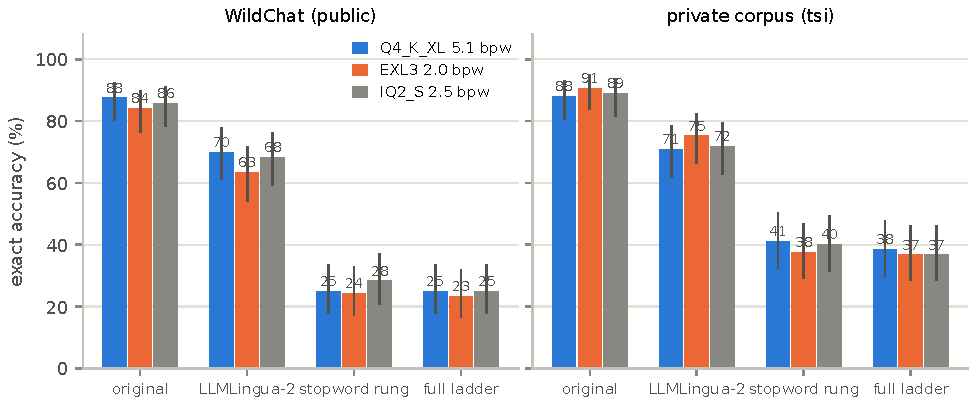
\includegraphics[width=\textwidth]{fig_grid.pdf}
\caption{Exact accuracy in all 24 cells, with 95\% Wilson intervals. In this
and the following figures, ``stopword rung'' is condition A and ``full ladder''
is condition E. Similar bar heights within a condition are descriptive;
overlapping marginal intervals are not a test of equality.}
\label{fig:grid}
\end{figure}

\begin{table}[t]
\centering
\small
\setlength{\tabcolsep}{4.5pt}
\begin{tabular}{llcccc}
\toprule
Corpus & Deployment & O & L2 & A & E \\
\midrule
\multirow{3}{*}{WildChat ($n=\PtwoWcItems$)}
 & Q4\_K\_XL & \PtwoAccQfWcO\ [\PtwoLoQfWcO,\PtwoHiQfWcO] & \PtwoAccQfWcL\ [\PtwoLoQfWcL,\PtwoHiQfWcL] & \PtwoAccQfWcA\ [\PtwoLoQfWcA,\PtwoHiQfWcA] & \PtwoAccQfWcE\ [\PtwoLoQfWcE,\PtwoHiQfWcE] \\
 & EXL3 2.0 & \PtwoAccExWcO\ [\PtwoLoExWcO,\PtwoHiExWcO] & \PtwoAccExWcL\ [\PtwoLoExWcL,\PtwoHiExWcL] & \PtwoAccExWcA\ [\PtwoLoExWcA,\PtwoHiExWcA] & \PtwoAccExWcE\ [\PtwoLoExWcE,\PtwoHiExWcE] \\
 & IQ2\_S & \PtwoAccIqWcO\ [\PtwoLoIqWcO,\PtwoHiIqWcO] & \PtwoAccIqWcL\ [\PtwoLoIqWcL,\PtwoHiIqWcL] & \PtwoAccIqWcA\ [\PtwoLoIqWcA,\PtwoHiIqWcA] & \PtwoAccIqWcE\ [\PtwoLoIqWcE,\PtwoHiIqWcE] \\
\midrule
\multirow{3}{*}{private ($n=\PtwoTsiItems$)}
 & Q4\_K\_XL & \PtwoAccQfTsiO\ [\PtwoLoQfTsiO,\PtwoHiQfTsiO] & \PtwoAccQfTsiL\ [\PtwoLoQfTsiL,\PtwoHiQfTsiL] & \PtwoAccQfTsiA\ [\PtwoLoQfTsiA,\PtwoHiQfTsiA] & \PtwoAccQfTsiE\ [\PtwoLoQfTsiE,\PtwoHiQfTsiE] \\
 & EXL3 2.0 & \PtwoAccExTsiO\ [\PtwoLoExTsiO,\PtwoHiExTsiO] & \PtwoAccExTsiL\ [\PtwoLoExTsiL,\PtwoHiExTsiL] & \PtwoAccExTsiA\ [\PtwoLoExTsiA,\PtwoHiExTsiA] & \PtwoAccExTsiE\ [\PtwoLoExTsiE,\PtwoHiExTsiE] \\
 & IQ2\_S & \PtwoAccIqTsiO\ [\PtwoLoIqTsiO,\PtwoHiIqTsiO] & \PtwoAccIqTsiL\ [\PtwoLoIqTsiL,\PtwoHiIqTsiL] & \PtwoAccIqTsiA\ [\PtwoLoIqTsiA,\PtwoHiIqTsiA] & \PtwoAccIqTsiE\ [\PtwoLoIqTsiE,\PtwoHiIqTsiE] \\
\bottomrule
\end{tabular}
\caption{Exact accuracy (\%) and 95\% Wilson intervals. Original-condition
point estimates range from \PtwoOAccMin\% to \PtwoOAccMax\%.}
\label{tab:grid}
\end{table}

\subsection{No cross-tier interaction was detected}\label{sec:interaction}

Table~\ref{tab:interaction} reports the paired cross-tier estimand. Estimates
range from $\PtwoInterDeltaMin$ to \PtwoInterDeltaMax{} points, no contrast is
rejected by the Holm familywise rule, and all pointwise 95\% intervals include
zero. Their full envelope is $\PtwoInterCiLowMin$ to \PtwoInterCiHighMax{}
points. This envelope summarizes the individual intervals; it is neither a
simultaneous confidence bound nor a minimum detectable effect. The data show
similar observed compression costs but leave practically important interactions
unresolved. They do not establish independence or equivalence.

\begin{table}[t]
\centering
\small
\begin{tabular}{llcrrr}
\toprule
Corpus & Condition & Low tier & Interaction pp [95\% CI] & CR2 $p$ & Holm $p$ \\
\midrule
WildChat & L2 & EXL3 & $\PtwoIntWcLEx$\ [$\PtwoIntLoWcLEx$, $\PtwoIntHiWcLEx$] & \PtwoIntPWcLEx & \PtwoIntPHolmWcLEx \\
 & L2 & IQ2\_S & $\PtwoIntWcLIq$\ [$\PtwoIntLoWcLIq$, $\PtwoIntHiWcLIq$] & \PtwoIntPWcLIq & \PtwoIntPHolmWcLIq \\
 & A & EXL3 & $\PtwoIntWcAEx$\ [$\PtwoIntLoWcAEx$, $\PtwoIntHiWcAEx$] & \PtwoIntPWcAEx & \PtwoIntPHolmWcAEx \\
 & A & IQ2\_S & $\PtwoIntWcAIq$\ [$\PtwoIntLoWcAIq$, $\PtwoIntHiWcAIq$] & \PtwoIntPWcAIq & \PtwoIntPHolmWcAIq \\
 & E & EXL3 & $\PtwoIntWcEEx$\ [$\PtwoIntLoWcEEx$, $\PtwoIntHiWcEEx$] & \PtwoIntPWcEEx & \PtwoIntPHolmWcEEx \\
 & E & IQ2\_S & $\PtwoIntWcEIq$\ [$\PtwoIntLoWcEIq$, $\PtwoIntHiWcEIq$] & \PtwoIntPWcEIq & \PtwoIntPHolmWcEIq \\
\midrule
private & L2 & EXL3 & $\PtwoIntTsiLEx$\ [$\PtwoIntLoTsiLEx$, $\PtwoIntHiTsiLEx$] & \PtwoIntPTsiLEx & \PtwoIntPHolmTsiLEx \\
 & L2 & IQ2\_S & $\PtwoIntTsiLIq$\ [$\PtwoIntLoTsiLIq$, $\PtwoIntHiTsiLIq$] & \PtwoIntPTsiLIq & \PtwoIntPHolmTsiLIq \\
 & A & EXL3 & $\PtwoIntTsiAEx$\ [$\PtwoIntLoTsiAEx$, $\PtwoIntHiTsiAEx$] & \PtwoIntPTsiAEx & \PtwoIntPHolmTsiAEx \\
 & A & IQ2\_S & $\PtwoIntTsiAIq$\ [$\PtwoIntLoTsiAIq$, $\PtwoIntHiTsiAIq$] & \PtwoIntPTsiAIq & \PtwoIntPHolmTsiAIq \\
 & E & EXL3 & $\PtwoIntTsiEEx$\ [$\PtwoIntLoTsiEEx$, $\PtwoIntHiTsiEEx$] & \PtwoIntPTsiEEx & \PtwoIntPHolmTsiEEx \\
 & E & IQ2\_S & $\PtwoIntTsiEIq$\ [$\PtwoIntLoTsiEIq$, $\PtwoIntHiTsiEIq$] & \PtwoIntPTsiEIq & \PtwoIntPHolmTsiEIq \\
\bottomrule
\end{tabular}
\caption{Marginal paired difference-in-differences against the
higher-footprint deployment. Positive values mean the compressed condition
cost more at the low tier. Intervals use a source-conversation-clustered CR2
variance estimate and are pointwise; $p$ is the two-sided
Satterthwaite-reference value and Holm $p$ its step-down adjustment. The exact
cluster-sign-symmetry calculation is secondary and is not shown. These are not
equivalence tests.}
\label{tab:interaction}
\end{table}

\subsection{Compressor choice is the dominant observed effect}\label{sec:compressor}

\begin{table}[t]
\centering
\small
\setlength{\tabcolsep}{5pt}
\begin{tabular}{llccc}
\toprule
Corpus & Deployment & $\Delta$ L2 [CI] & $\Delta$ A [CI] & $\Delta$ E [CI] \\
\midrule
\multirow{3}{*}{WildChat}
 & Q4\_K\_XL & \PtwoDelQfWcL\ [\PtwoDloQfWcL,\PtwoDhiQfWcL] & \PtwoDelQfWcA\ [\PtwoDloQfWcA,\PtwoDhiQfWcA] & \PtwoDelQfWcE\ [\PtwoDloQfWcE,\PtwoDhiQfWcE] \\
 & EXL3 2.0 & \PtwoDelExWcL\ [\PtwoDloExWcL,\PtwoDhiExWcL] & \PtwoDelExWcA\ [\PtwoDloExWcA,\PtwoDhiExWcA] & \PtwoDelExWcE\ [\PtwoDloExWcE,\PtwoDhiExWcE] \\
 & IQ2\_S & \PtwoDelIqWcL\ [\PtwoDloIqWcL,\PtwoDhiIqWcL] & \PtwoDelIqWcA\ [\PtwoDloIqWcA,\PtwoDhiIqWcA] & \PtwoDelIqWcE\ [\PtwoDloIqWcE,\PtwoDhiIqWcE] \\
\midrule
\multirow{3}{*}{private}
 & Q4\_K\_XL & \PtwoDelQfTsiL\ [\PtwoDloQfTsiL,\PtwoDhiQfTsiL] & \PtwoDelQfTsiA\ [\PtwoDloQfTsiA,\PtwoDhiQfTsiA] & \PtwoDelQfTsiE\ [\PtwoDloQfTsiE,\PtwoDhiQfTsiE] \\
 & EXL3 2.0 & \PtwoDelExTsiL\ [\PtwoDloExTsiL,\PtwoDhiExTsiL] & \PtwoDelExTsiA\ [\PtwoDloExTsiA,\PtwoDhiExTsiA] & \PtwoDelExTsiE\ [\PtwoDloExTsiE,\PtwoDhiExTsiE] \\
 & IQ2\_S & \PtwoDelIqTsiL\ [\PtwoDloIqTsiL,\PtwoDhiIqTsiL] & \PtwoDelIqTsiA\ [\PtwoDloIqTsiA,\PtwoDhiIqTsiA] & \PtwoDelIqTsiE\ [\PtwoDloIqTsiE,\PtwoDhiIqTsiE] \\
\bottomrule
\end{tabular}
\caption{Paired percentage points lost relative to original context, with
95\% Newcombe method-10 intervals. The per-cell exact McNemar $p$-values are
computed in the released claims file rather than tabulated here; they
establish damage relative to O, not equality across tiers.}
\label{tab:deltas}
\end{table}

\begin{figure}[t]
\centering
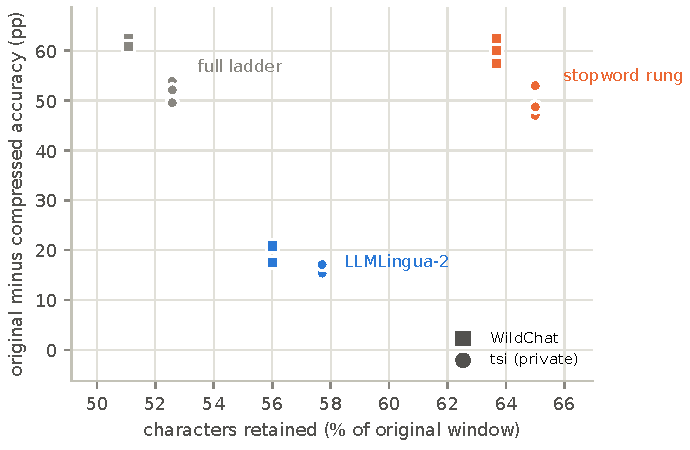
\includegraphics[width=0.62\textwidth]{fig_ratio.pdf}
\caption{Paired accuracy cost against aggregate character retention. Six
points per condition represent three tiers in each corpus.}
\label{fig:ratio}
\end{figure}

Table~\ref{tab:deltas} reports the paired within-deployment costs, and
Figure~\ref{fig:ratio} plots each cost against character retention.
LLMLingua-2 retains \PtwoRetLWc\% of characters in the public arm
(\PtwoRetLTsi\% private) and costs \PtwoLDelMin--\PtwoLDelMax{} points. The
deterministic rungs retain \PtwoRetEWc--\PtwoRetAWc\% publicly
(\PtwoRetETsi--\PtwoRetATsi\% private) and cost
\PtwoNaiveDelMin--\PtwoNaiveDelMax{} points. Retention fraction alone
therefore does not predict QA damage in this grid. The strongest comparison is
L2 against E: their requested per-window rates are matched, yet their accuracy
costs differ by tens of points. This supports evaluating the compressor on the
downstream task rather than treating character ratio or embedding similarity
as a sufficient quality measure.

\subsection{Serving throughput after compression}\label{sec:timing}

\begin{figure}[t]
\centering
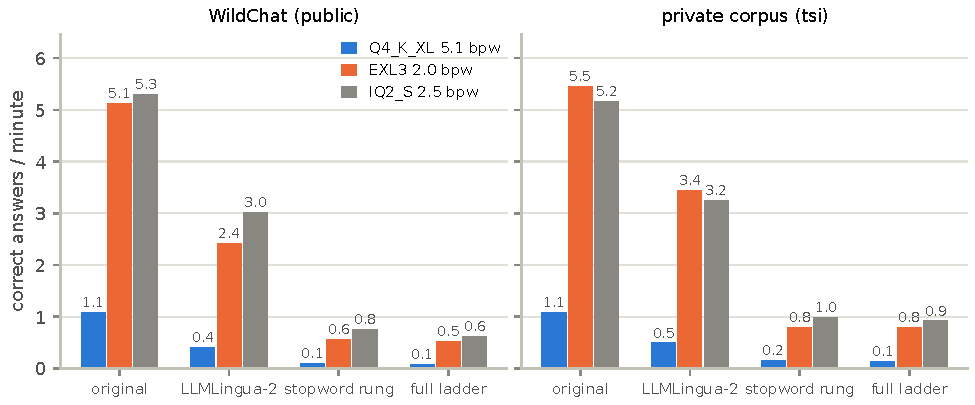
\includegraphics[width=\textwidth]{fig_accmin.pdf}
\caption{Correct answers per model-serving minute. Compressor preprocessing is
excluded. The figure is descriptive and does not identify the timing
mechanism.}
\label{fig:accmin}
\end{figure}

Figure~\ref{fig:accmin} plots correct answers per model-serving minute.
Original contexts produce \PtwoApmOMin--\PtwoApmOMax{} exact-correct answers
per model-serving minute across the six deployment--corpus pairs. LLMLingua-2
produces \PtwoApmLMin--\PtwoApmLMax{}, and the naive conditions produce
\PtwoApmNaiveMin--\PtwoApmNaiveMax{}. Mean request time is
\PtwoWallOMin--\PtwoWallOMax{} seconds for O and
\PtwoWallNaiveMin--\PtwoWallNaiveMax{} seconds for the naive conditions;
per-cell means for every condition, including L2, are in the released claims
file. The analysis does not use the stored usage telemetry, and no per-token
timing series exists, so whether the difference comes from prefill, decode
length, decode rate, or another server behavior is left unresolved; the
measurement also omits the offline compression pass. The supported statement
is therefore limited: for these already-fitting inputs, within each of the six
deployment--corpus pairs, every compressed condition yields fewer correct
answers per recorded serving minute than the original context, and its mean
request time is longer. The pooled ranges above overlap only because the
higher-footprint deployment is slower than either low tier under every
condition. It does not
imply that compression cannot
improve latency for longer prompts or other hardware; controlled studies find
such gains in matched operating windows \citep{kummer2026wild}.

\subsection{Operational answer survival}\label{sec:survival}

\begin{figure}[t]
\centering
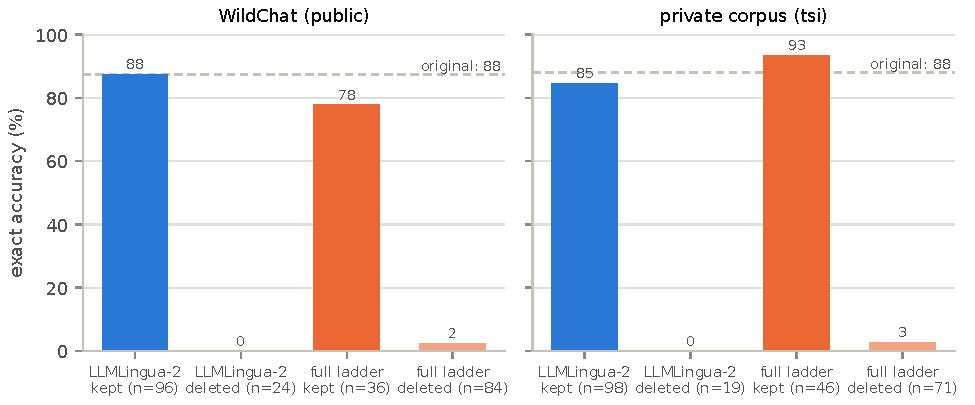
\includegraphics[width=\textwidth]{fig_survival.pdf}
\caption{Exact accuracy conditional on the operational answer-survival tag for
the higher-footprint deployment. ``Deleted'' means the normalized gold no
longer occurs in the identically normalized compressed text under the frozen
survival rule.}
\label{fig:survival}
\end{figure}

Figure~\ref{fig:survival} conditions accuracy on the survival tag. The
survival covariate marks a gold answer as present when its normalized form
(case-folded, whitespace-collapsed, with quote, backtick, bracket, and
punctuation edges trimmed) occurs in the identically normalized compressed
text. Under that operational rule, applied to the L2 and E conditions (the
covariate is not computed for A), \PtwoDestPairs{} unique item--condition
pairs are tagged deleted. Each is
evaluated at all three tiers, producing \PtwoDestTrials{} tier-level
evaluations, of which \PtwoDestRecovered{} are exact-correct. This is an
observed count, not proof about what reconstruction is possible.

LLMLingua-2 retains the operational gold in
\PtwoSurvWcLN/\PtwoSurvWcLTot{} public items
(\PtwoSurvWcLPct\%; private \PtwoSurvTsiLPct\%), and exact accuracy among
survivors is \PtwoSurvAccLMin--\PtwoSurvAccLMax\%. E retains the gold in
\PtwoSurvWcEPct\% of public items (private \PtwoSurvTsiEPct\%), with survivor
accuracy of \PtwoSurvAccEMin--\PtwoSurvAccEMax\%. Answer availability and the
structure needed to locate an answer are therefore both part of compression
damage in this grid.

\subsection{Public and private arms}

Both arms show the same descriptive ordering of conditions at every
deployment, with O above L2 and L2 above both naive rungs, and neither arm
contributes a contrast that the Holm rule rejects. The L2 cell accuracies span
\PtwoLAccMin--\PtwoLAccMax\% across both arms. This agreement is useful
robustness evidence, but it is not a formal equivalence or replication test.
Every central direction is visible in the public arm; the private arm adds
only aggregate evidence from one motivating workload.

\section{Discussion}\label{sec:discussion}

The principal result is modest but operationally useful. Within one
extractive-QA design, switching among the three deployed tiers did not reveal
a larger penalty for compressed context. The interaction point estimates are
small relative to the condition effects reported in \S\ref{sec:compressor}.
For a practitioner using these exact stacks, the evidence favors validating
the compressor over choosing a different compressor for each tier.

The uncertainty limits that recommendation. The pointwise intervals span
$\PtwoInterCiLowMin$ to \PtwoInterCiHighMax{} points across the comparisons;
none defines a study-wide detection threshold. An operator who needs to rule
out a consequential extra loss should pre-specify an acceptable margin and
power an equivalence or non-inferiority study, ideally on tasks with
meaningfully different clean-input performance across tiers.

The artifact--engine framing also matters. The lower-footprint tiers are fully
GPU resident; the higher-footprint GGUF is partially offloaded. The study asks
whether compression cost is robust across those useful deployment choices. It
does not support a weight-precision causal claim: no single component of the
deployment stack receives attribution.

Finally, compression is not interchangeable with capacity in this evidence.
Character retention is only a rough input-size measure, all requests already
fit, and the context allocation is fixed. The grid measures the cost of
discarding input that could have been kept. Whether compression is beneficial
when it makes an otherwise impossible request fit is a different experiment.

\section{Limitations}\label{sec:limits}

The corrective chronology is the first limitation: P2R1 was designed after the
hypotheses, corpus frames, and contaminated outputs of the quarantined
campaign had been observed. Fresh seeded questions and an identity-verified
harness repair the measurement chain, but the study remains a corrected
measurement rather than a replication, and its inferences condition on one
frozen question set and one sampled decode per cell. The EXL3 server did not
apply the requested evaluation seed, and the study does not estimate
decode-to-decode variability.

The evidence covers one dense 27B checkpoint, one laptop, three deployed
artifact--engine--placement configurations, and short-answer extractive QA.
Reasoning, synthesis, tool use, and generation-heavy tasks may show a
different interaction. Because engine, format, effective precision, footprint,
and GPU residency co-vary, no component receives a causal attribution.

The interaction intervals are pointwise and remain wide; no equivalence margin
or power target was specified.
Original-condition accuracy is high
(\PtwoOAccMin--\PtwoOAccMax\%), which reduces room to observe compression
helping. Questions were generated by the higher-footprint deployment, creating
possible selection advantage for that tier. The private long/no-code stratum
contains only 6 windows, so long-context claims rest mostly on the other
strata. Timing is observational within item-interleaved server sessions and
supports serving-time descriptions, not a mechanism. Character retention does
not measure token retention or KV memory. Prompt injection in source
conversations was not separately scored and could affect the exact-answer
protocol.

The private corpus cannot be released. WildChat is available under ODC-By, but
that database license does not necessarily clear independent rights in every
conversation, so raw windows, excerpts, questions, answers, and responses stay
private in both arms and only aggregate statistics are released.

\section{Reproducibility and data availability}\label{sec:repro}

All reported numbers derive from a single promotion record binding the frozen
outputs to the protocol, harness hashes, server-identity and placement checks,
host inventory, and artifact/CUDA-runtime receipts. Rebuilding claims also
verifies that chain. Exact model artifacts are identified by upstream
repository, immutable revision, filename, byte count, SHA-256, and license.

Question generation uses the separate llama.cpp Q4 endpoint with the fixed
seed schedule above; source selection and item ordering are also seeded.
These controls do not make the EXL3 evaluations reproducible from seed 42.
Analysis reproduction instead uses the exact saved outputs. The generated
questions and gold answers are
derivatives of conversation content: releasing them requires a separate rights
and privacy decision, so the public package contains aggregate statistics,
builder and analysis code, environment records, and provenance receipts rather
than raw text.
The accompanying aggregate artifact, version 1.0.0, is identified by
\href{https://doi.org/\PtwoArtifactDOI}{doi:\PtwoArtifactDOI}.
For analysis-only reproduction, run \q{python3 check\_claims.py} at the artifact
root. The standard-library verifier recomputes the reported intervals, tests,
Holm decisions, and manuscript numbers from aggregate cluster histograms;
it needs no model, GPU, or network access. Full inference replication is a
separate task: \q{FULL\_RERUN.md} specifies the pinned artifacts, environment,
and harness commands. External reruns must regenerate public questions and
cannot reproduce the unreleased private corpus.

\section{Ethics and disclosure}

WildChat's maintainers report de-identification and removal of identified
sensitive conversations, but residual sensitive material remains possible in
real-world chat logs. No conversation text is quoted in the manuscript or
included in the public release. Private assistant-chat material is reported
only as aggregates and was scanned against release text.

\noindent\textbf{AI assistance.} Claude (Anthropic) and Codex (OpenAI)
assisted with evaluation-harness development, experiment orchestration,
evidence auditing, analysis and figure code, citation checking, and
manuscript drafting and revision. Matthew Schwartz directed the research and
is responsible for its methods, results, interpretation, claims, citations,
rights, and released artifacts.

\section{Conclusion}

Across three real deployments of one 27B checkpoint, this corrective
exploratory rerun detected no cross-tier accuracy interaction between
quantization tier and lossy context compression on paired extractive QA. The
estimated differences in compression cost are $\PtwoInterDeltaMin$ to
\PtwoInterDeltaMax{} points, no contrast survives the Holm familywise rule,
and the pointwise interval envelope is $\PtwoInterCiLowMin$ to
\PtwoInterCiHighMax{} points. The result is therefore a bounded non-detection,
not proof of
independence. Within the same grid, compressor choice changes accuracy by tens
of points: LLMLingua-2 loses far less than a stopword/code-stripping pipeline
at similar character retention. For these already-fitting inputs, the original
context also yields the most correct answers per recorded serving minute on
every deployment. The
practical lesson is to validate context transformations on the actual
downstream task and deployed stack. Claims that any extra loss is acceptably
small require a separate, adequately powered equivalence design.

\bibliographystyle{plainnat}
\bibliography{references}

\end{document}
